\documentclass[aspectratio=169, 12pt]{beamer}
% \documentclass[aspectratio=169, handout]{beamer} % for handout
\usepackage{pgfpages}
\usepackage[english]{babel}
\usepackage{booktabs,listings}
\usepackage[T1]{fontenc}
\usepackage[utf8]{inputenc}
\usepackage{xcolor}
\usepackage{graphicx}
\usepackage{graphics}
\usepackage{epstopdf}
\usepackage{upgreek}
\usepackage{amsmath}
\usepackage{textcomp}
\usepackage{booktabs}
\usepackage{tikz}
\usetikzlibrary{positioning,shapes,arrows,calc}
\usepackage{adjustbox}
\usepackage{siunitx}
\newcommand{\mesunt}[1]{\left[\si{#1}\right]}

\lstset{basicstyle=\ttfamily}
\setlength{\parskip}{.5\baselineskip}
\usetheme[style=vertical, frametotal=true]{NTNU}

\mode<handout>{%
    \pgfpagesuselayout{2 on 1}[a4paper] 
    % \setbeameroption{show notes}
}

\AtBeginSection[]
{
  \begin{frame}
    \frametitle{Table of Contents}
    \tableofcontents[currentsection]
  \end{frame}
}

\title{ Repartition of inertia service between wind turbine and battery in power systems }
% \subtitle{Project for the ET8301 course}
\author{Andreetta Niccolò}
\date{May $31^{st}$ 2024}

\begin{document}
  \maketitle

  \begin{frame}[fragile]{Outline}
    \tableofcontents
  \end{frame}

  \begin{frame}
    \begin{itemize}
      \item Lost of inertia problem: Implication of converter interfaced devices and so lost of inertia
      \item New metrics: how can we evaluate the performance of the grid with the inclusion of this devices, since it is possible that the old one are no more able to characterize it sufficiently
      \item How can we counteract to this lost of inertia: what's the inertia provision service, how can it be provided at market level (and possibly in APS)
      \item Grid Forming and Following: how can we operate the electronic in grid forming and following mode for providing stability to the grid
    \end{itemize}
  \end{frame}

  \section{Background and problem statement}
  \begin{frame}{\insertsection}
    Increase of energy from renewable energy resources implies lost of inertia in the grid. 

  \end{frame}
  
  \section{Research questions}
  \begin{frame}{Research questions}
    \textcolor{NTNUBlue}{Main question}: Which is the most effective way to provide inertia when a wind turbine and a battery are available in a power system?
    
    \textcolor{NTNUOrange}{Solution idea}: Allocate the amount of power between the available in the most economic way
  \end{frame}

  \section{Metrics}
  \begin{frame}{Time domain of the post-fault frequency evolution}{Classical metrics}
    \begin{itemize}[<+(1)->]
      \item Rate of Change of Frequency
      \begin{equation}
        \lvert \dot{\omega} \rvert _{max} = \max_i\left(\max_{t\ge0}\lvert \dot{\omega}_i(t) \rvert\right)
      \end{equation}
      
      \item Frequency Nadir
      \begin{equation}
        \lvert \underline{\omega} \rvert = \max_i\lvert\min_{t\ge0} \omega_i(t) \rvert
      \end{equation}
      \item Peak virtual inertia power injection
      \begin{equation}
        \bar{p}_v = \max_i\left(\max_{t\ge0}\lvert p_{v,i}(t) \rvert\right)
      \end{equation}
    \end{itemize}
  \end{frame}

  \begin{frame}{Time domain of the post-fault frequency evolution}{Energy metrics}
    \begin{itemize}[<+(1)->]
        \item Total energy imbalance
        \begin{equation}
          E_{\tau,\omega}=\int_{0}^{\tau}\sum_{i} q_i\omega_i^{2}dt=\int_{0}^{\tau} \omega^T Q \omega dt
        \end{equation}
        
        \item Total virtual inertia effort
        \begin{equation}
          E_{\tau,m}=\int_{0}^{\tau}\sum_{i} r_{m,i}p_{m,i}^{2}dt=\int_{0}^{\tau} p_{m}^T R_m p_{m} dt
        \end{equation}

        \item Total virtual damping effort
        \begin{equation}
          E_{\tau,d}=\int_{0}^{\tau}\sum_{i} r_{d,i}p_{d,i}^{2}dt=\int_{0}^{\tau} p_{d}^T R_d p_{d} dt
        \end{equation}
      \end{itemize}

      $q_i, r_m, and r_d$ are weights used for penalize one effort or the other
  \end{frame}
  
  \begin{frame}
    Eigenvalue analysis
    \begin{itemize}
      \item Damping ratio of the power system
      \begin{equation}
        \zeta_{min} = \min_{k}\frac{-\sigma_k}{\sqrt{\sigma_k^2 + \omega_k^2}}
      \end{equation}
      with $\lambda_k=\sigma_k + \text{i}\omega_k$ the $k-th$ eigenvalue
    \end{itemize}
    
    Physical and virtual inertia of the devices
  \begin{itemize}
    \item Total inertia
    \begin{equation}
      H_{total} = \sum_{i}H_i + \sum_{i} \tilde{H}_i = \sum_{i}\frac{m_i \omega_0}{2 S_{rated,i}} + \sum_{i} \frac{\tilde{m}_i \omega_0}{2 S_{rated,i}}
    \end{equation} 
  \end{itemize}
\end{frame}

\begin{frame}
  \begin{itemize}[<+(1)->]
    \item $\mathcal{H}_2$ norm: energy of the response to an impulse fault \textit{or} expected energy of the response to a white noise
    \begin{equation}
      \int_{0}^{\infty}\| y_p \|^2 dt = \int_{0}^{\infty} \omega^T Q \omega + p_{m}^T R_m p_{m} + p_{d}^T R_d p_{d} dt
    \end{equation}
    \textcolor{NTNUViolet}{
    Example: 
    \begin{gather}
      \text{System } \mathcal{G} :
      \begin{cases}
        \dot{x} = A x + G \eta \\
        y_p = C x
      \end{cases}
      \Rightarrow \| \mathcal{G} \|_2^2=\text{trace}\left(G^T P G\right)\\
      \text{Observability gramian: } PA + A^TP+C^TC=0
    \end{gather} 
    }
    \item $\mathcal{H}_{\infty }$ norm: root mean square gain from the disturbance to the performance output
  \end{itemize}
\end{frame}

\begin{frame}{Use of the metrics}
  Test on the Kundor model with two different damping configuration
  \begin{columns}
    \begin{column}{0.5\columnwidth}
      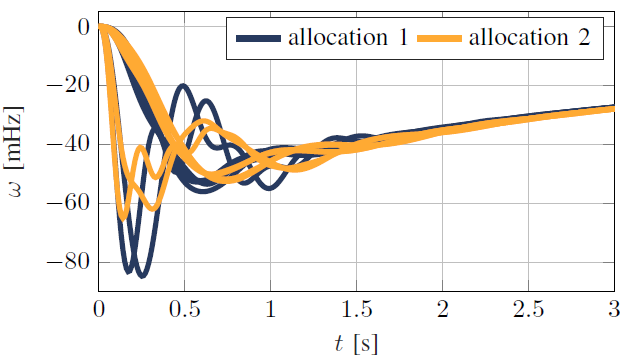
\includegraphics[width = \columnwidth]{figure/kundor_frequency.png}
    \end{column}
    \begin{column}{0.5\columnwidth}
      \begin{table}[h!]
        \centering
        \begin{tabular}{lcc}
        \toprule
        & Allocation 1 & Allocation 2 \\
        \midrule
        $H_{\text{total}}$ & 40.85 s & 40.85 s \\
        $\zeta_{\text{min}}$ & 0.1190 & 0.1206 \\
        $\left|\dot{\omega}\right|_{\max}$ & 0.8149 Hz/s & 0.8135 Hz/s \\
        $\left|\omega\right|$ & 84.8 mHz & 65.1 mHz \\
        $\mathcal{H}_2 $ & 1.5337 & 0.6522 \\
        $\mathcal{H}_{\infty} $ & 0.7454 & 0.2782 \\
        $\overline{P}_v$ & 118.38 MW & 7.0446 MW \\
        \bottomrule
        \end{tabular}
      
        \label{table:allocations}
        \end{table}
    \end{column}
  \end{columns}
\end{frame}

\section{Inertia market}  
\begin{frame}
  
\end{frame}

\end{document}